\documentclass[12pt]{article}
\usepackage[paper=letterpaper,margin=2cm]{geometry}
\usepackage{amsmath}
\usepackage{amssymb}
\usepackage{amsfonts}
\usepackage{graphicx}
\graphicspath{ {./images/} }
\usepackage{newtxtext, newtxmath}
\usepackage{enumitem}
\usepackage{titling}
\usepackage[colorlinks=true]{hyperref}
\usepackage[spanish]{babel}

\setlength{\droptitle}{-6em}

% Enter the specific assignment number and topic of that assignment below, and replace "Your Name" with your actual name.
\title{Práctica 2 - Programación Concurrente y de Tiempo Real}
\author{Víctor Moreno Sola}
\date{\today}

\begin{document}
\maketitle

\textbf{Ejercicio 3 - escalaVector.java, escalaVPar.java y tablaCPU.java}
\\
\\En las próximas figuras observaremos los picos de uso de la CPU cuando ejecutamos las dos versiones on tamaños de vector de 1.000.000.000 de posiciones.

    \begin{figure}[h!]
        \centering
        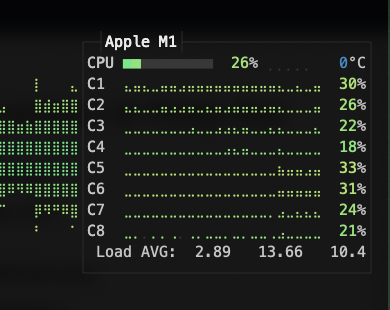
\includegraphics[scale=0.5]{images/psecuencial1000000000.png}
        \caption{Pico de uso de CPU en la versión secuencial}
        \label{fig:my_label}
    
        \vspace{1cm}
        
        \centering
        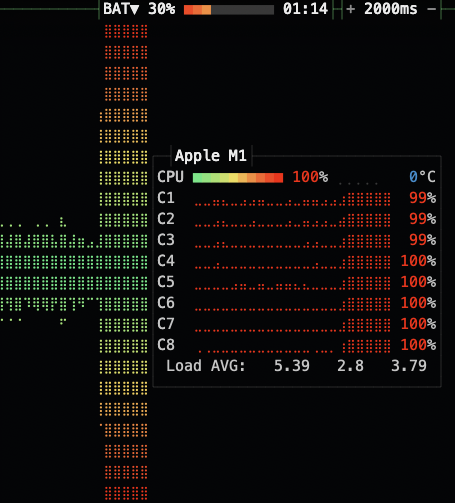
\includegraphics[scale=0.4]{paralelo1000000000}
        \caption{Pico de uso de CPU en la versión paralelizada}
        \label{fig:my_label}
        
    \end{figure}   
        


Como podemos observar en Figura 1, apenas se sobrecargan los diferentes núcleos del procesador mientras que en Figura 2, la versión paralelizada, al crear 8 hilos son los 8 núcleos los que se encargan del procesado del programa llegando al máximo de sus posibilidades.

\end{document}
